\subsection{Curvilinear Geometry Base Class}
\label{interface-curvilineargeometry}

\noindent
Curvilinear Geometry can be initialized either using the interpolator class, or the parameters necessary to initialize the interpolator class \\

\begin{mybox}
\begin{lstlisting}
  CurvilinearGeometry ( const ElementInterpolator & elemInterp)
  CurvilinearGeometry ( const ReferenceElement &refElement, const Vertices &vertices, InterpolatoryOrderType order)
  CurvilinearGeometry ( Dune::GeometryType gt, const Vertices &vertices, InterpolatoryOrderType order)
\end{lstlisting}
\end{mybox}

\noindent
Standard dune functionality \\
\begin{mybox}
\begin{lstlisting}
  bool affine ()
  GlobalCoordinate center ()
\end{lstlisting}
\end{mybox}

\noindent
Wrapper for basic interpolator functionality \\
\begin{mybox}
\begin{lstlisting}
  InterpolatoryOrderType order()
  Dune::GeometryType type()
  int nCorner ()
  int nVertex ()
  GlobalCoordinate corner ( InternalIndexType cornerLinearIndex )
  GlobalCoordinate vertex (int i)
  std::vector< GlobalCoordinate > cornerSet()
  std::vector<GlobalCoordinate> vertexSet()
\end{lstlisting}
\end{mybox}

\noindent
Wrapper for extended interpolator functionality \\
\begin{mybox}
\begin{lstlisting}
  ElementInterpolator interpolator()
  PolynomialVector interpolatoryVectorAnalytical()

  template<int subdim>
  CurvilinearGeometry< ctype, subdim, cdim>  subentityGeometry(InternalIndexType subentityIndex)
\end{lstlisting}
\end{mybox}

\noindent
Mappings \\
\begin{mybox}
\begin{lstlisting}
  GlobalCoordinate global ( const LocalCoordinate &local )
  bool local ( const GlobalCoordinate &globalC, LocalCoordinate & localC )
\end{lstlisting}
\end{mybox}

\noindent
Construction of normals \\
\begin{mybox}
\begin{lstlisting}
  GlobalCoordinate normal(const LocalCoordinate &local )
  GlobalCoordinate subentityNormal(InternalIndexType indexInInside, const LocalCoordinate &local )
  GlobalCoordinate subentityUnitNormal(InternalIndexType indexInInside, const LocalCoordinate &local )
  GlobalCoordinate subentityIntegrationNormal(InternalIndexType indexInInside, const LocalCoordinate &local )
\end{lstlisting}
\end{mybox}

%\noindent
%Construction numerical and analytic integration elements. \\

%\noindent
%\uline{JacobianDeterminantAnalytical}: $|\det J_{ij}|$ is available explicitly in polynomial form, when $(dim_{elem} = dim_{world})$. Although modulus is not a polynomial operation, $\det J_{ij} \neq 0$ inside the element, because the geometry must not be self-intersecting. Hence $\det J_{ij}$ is not allowed to change sign within the element, and modulus-correction is to evaluate $\det J_{ij}$ anywhere inside the element and multiply the analytic expression by $-1$ if the result is negative. \\

%\noindent
%\uline{NormalIntegrationElementAnalytical}: Surface normal integration element $d\vec{S} = \vec{n} dS $ is available. For edges in 2D defined by $d\vec{l} = (\partial_u p_y, -\partial_u p_x) du$. For triangles in 3D defined by $d \vec{S} = -(\partial_u \vec{p} \times \partial_v \vec{p}) du dv $ \\

%\noindent
%\uline{IntegrationElementSquaredAnalytical}: The square of the pseudodeterminant $\det(JJ^T)$, when $(dim_{elem} \neq dim_{world})$. For edges this expression is equal to $|\partial_u \vec{p}|^2$. For triangles in 3D this expression is equal to $|\vec{dS} / (du \; dv)|^2$. \\



\noindent
Numeric integration provided via standard integration elements, that can be further used in a quadrature routine. An exception to the interface is the volume method, which has do be done recursively, since the integration element need not be polynomial. Here, CurvilinearGeometry directly uses the recursive quadrature, and thus requires a tolerance parameter to terminate.

\begin{mybox}
\begin{lstlisting}
  ctype integrationElement ( const LocalCoordinate &local )
  JacobianTransposed jacobianTransposed ( const LocalCoordinate &local )
  JacobianInverseTransposed jacobianInverseTransposed ( const LocalCoordinate &local )
  ctype volume (double tolerance)
\end{lstlisting}
\end{mybox}




%\subsubsection{Methods - Cached Lagrange Geometry}
%\label{interface-curvilineargeometry-cached-methods}



\subsubsection{Tests}

\noindent
We start by explicitly defining the local-global mapping functors to mimic LagrangeGeometry for simplices of all 3 dimensions (Table 2). Then the following test procedure is run for each of the simplex mapping:
\begin{itemize}
	\item Loop over 5 interpolatory orders.
	\item For each order sample the interpolatory points from the mapping. Construct LagrangeGeometry and CurvilinearLagrangeGeometry classes.
	\item \textbf{Test 1}. To test if the Geometry has been correctly initialized, return all of its corners and check if they match those evaluated by the function.
	\item \textbf{Test 2}. To test local-to-global functionality, a random set of local points is sampled over the element, and the result of method $global()$ of the Geometry is compared with that of the explicit mapping. The test is omitted if the interpolation order is smaller than the order of the mapping.
	\item \textbf{Test 3}. To test global-to-local functionality, the local method is used for all the interpolation points expecting to obtain the points of the local interpolation grid over reference simplex. Also, it is checked if all these points are reported to be inside the element. This test fails a lot:
		\subitem -Fails to consider the point that is close to the boundary as in.
		\subitem -Fails to converge to a boundary point if the geometry has a zero derivative on the corner or on the whole boundary.
	\item \textbf{Test 4}. To test global-to-local using more probable sample points, the local coordinates are randomly sampled. It is then verified if $\vec{p} \approx local(global(\vec{p}))$. This test also checks if all the sample points are reported inside as they should be.
	\item \textbf{Test 5}. To check if the outside points are correctly sampled outside, as well as check the correctness of surface normal, we loop over all boundaries of the element, construct boundary normals for a uniform grid on the each boundary, and obtain the points which are just outside the element by calculating $\vec{p} = \vec{g} + \alpha \vec{n}$, where $\vec{g}$ is the global coordinate of of some point on the boundary, $\vec{n}$ is the normal at that point, and $\alpha = 0.01$ is a small number. \cref{fig:geometry:test:normal}.
	\item \textbf{Test 6}. The scalar basis functions given in Table 1 are integrated over the Geometry, and results are compared to those calculated by hand, given in Table 2.
	\item \textbf{Test 7}. The dot product surface integrals of vector basis functions (given in Table 3) over the Geometry are compared to those calculated by hand, given in Table 4.
\end{itemize}

\begin{figure}
    \centering
    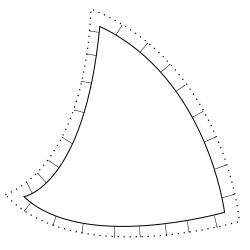
\includegraphics[scale=1.0]{images/normaltest}
	\captionsetup{width=0.8\textwidth} 
	\caption{ A combined test for normal accuracy and ability to accurately determine that a vertex is outside the element. Face normals sampled over a grid are used to produce global coordinates just outside the the element, which are then checked for having a local coordinate inside that element. }
	\label{fig:geometry:test:normal}
\end{figure}

\subsubsection{Integral-tests}

\begin{center}
\begin{tabular}{ | l | l | l |}
  \hline
  Ord & Dim & Scalar Basis Function \\ \hline
  0 & 1 & $1$ \\ \hline
  1 & 1 & $1 + 2x$ \\ \hline
  2 & 1 & $1 + 2x + 3x^2$ \\ \hline
  3 & 1 & $1 + 2x + 3x^2 + 4x^3$ \\ \hline
  4 & 1 & $1 + 2x + 3x^2 + 4x^3 + 5x^4$ \\ \hline
  5 & 1 & $1 + 2x + 3x^2 + 4x^3 + 5x^4 + 6x^5$ \\ \hline
%%  
  0 & 2 & $1$ \\ \hline
  1 & 2 & $1 + 2(x + y)$ \\ \hline
  2 & 2 & $1 + 2(x + y) + 3(x^2 + y^2) + xy$ \\ \hline
  3 & 2 & $1 + 2(x + y) + 3(x^2 + y^2) + xy + 4(x^3 + y^3) + xy^2$ \\ \hline
  4 & 2 & $\begin{array}{lcl} 1 & + & 2(x + y) + 3(x^2 + y^2) + xy + 4(x^3 + y^3) + xy^2 \\ & + & 5(x^4 + y^4) + xy^3 \end{array}$ \\ \hline
  5 & 2 & $\begin{array}{lcl} 1 & + & 2(x + y) + 3(x^2 + y^2) + xy + 4(x^3 + y^3) + xy^2 \\ & + & 5(x^4 + y^4) + xy^3 + 6(x^5 + y^5) + xy^4 \end{array}$ \\ \hline
%%  
  0 & 3 & $1$ \\ \hline
  1 & 3 & $1 + 2(x + y + z)$ \\ \hline
  2 & 3 & $1 + 2(x + y + z) + 3(x^2 + y^2 + z^2) + xy$ \\ \hline
  3 & 3 & $1 + 2(x + y + z) + 3(x^2 + y^2 + z^2) + xy + 4(x^3 + y^3 + z^3) + xyz$ \\ \hline
  4 & 3 & $\begin{array}{lcl} 1 & + & 2(x + y + z) + 3(x^2 + y^2 + z^2) + xy + 4(x^3 + y^3 + z^3) + xyz \\ & + & 5(x^4 + y^4 + z^4) + xyz^2 \end{array}$ \\ \hline
  5 & 3 & $\begin{array}{lcl} 1 & + & 2(x + y + z) + 3(x^2 + y^2 + z^2) + xy + 4(x^3 + y^3 + z^3) + xyz \\ & + & 5(x^4 + y^4 + z^4) + xyz^2 + 6(x^5 + y^5 + z^5) + xyz^3 \end{array}$ \\ \hline
\end{tabular}
\vfill
\title{Table 1. Scalar basis functions used, one of each polynomial order, one per geometry dimension}
\end{center}

\noindent
Using the vector basis functions $(x, x)$ for 2D edges and $(x, y, xy)$ for 3D triangles, we obtain the following integrals for the curvilinear maps

\begin{center}
\begin{tabular}{ | l | l | l | l | l | l | }
  \hline
  mydim & cdim & map               & Normal                  & Integrand                  & Result     \\ \hline
  1     & 2    & $(x,0)$           & $(0,-1)$                & $-x$                       & $-1/2$     \\ \hline
  1     & 2    & $(2x,3x)$         & $(3,-2)$                & $x$                        & $1/2$      \\ \hline
  1     & 2    & $(x,x^2)$         & $(2x,-1)$               & $2x^2-x$                   & $1/6$      \\ \hline
  2     & 3    & $(x,y,0)$         & $(0,0,-1)$              & $-xy$                      & $-1/24$    \\ \hline
  2     & 3    & $(y,3x,x+y)$      & $(-3,-1,3)$             & $-3x-y+3xy$                & $-13/24$   \\ \hline
  2     & 3    & $(y^2,x^2,xy)$    & $(-2y^2,-2x^2,4xy)$     & $-2x^3-2y^3+4x^2y^2$      & $-17/180$   \\ \hline
\end{tabular}
\\
\title{Table 3. DotProduct Integrals of Vector basis functions over curved boundaries}
\end{center}


\begin{landscape}

\begin{center}
\begin{tabular}{ | l | l | l | l | l | l | l | l | l |}
  \hline
  $d_e$ & Map & $\mu(\vec{r})$ & $I_0$ & $I_1$ & $I_2$ & $I_3$ & $I_4$ & $I_5$ \\ \hline
  1 & $(x)$                & $1$ & $1.0$ & $2.0$ & $3.0$ & $4.0$ & $5.0$ & $6.0$ \\ \hline
  1 & $(x,0)$              & $1$ & $1.0$ & $2.0$ & $3.0$ & $4.0$ & $5.0$ & $6.0$ \\ \hline
  1 & $(x,0,0)$            & $1$ & $1.0$ & $2.0$ & $3.0$ & $4.0$ & $5.0$ & $6.0$ \\ \hline
  1 & $(1+2x)$             & $2$ & $2.0$ & $4.0$ & $6.0$ & $8.0$ & $10.0$ & $12.0$ \\ \hline
  1 & $(2x,3x)$            & $\sqrt{13}$ & $\sqrt{13}$ & $2\sqrt{13}$ & $3\sqrt{13}$ & $4\sqrt{13}$ & $5\sqrt{13}$ & $6\sqrt{13}$ \\ \hline
  1 & $(2x,0.5+3x,5x)$     & $\sqrt{38}$ & $1\sqrt{38}$ & $2\sqrt{38}$ & $3\sqrt{38}$ & $4\sqrt{38}$ & $5\sqrt{38}$ & $6\sqrt{38}$ \\ \hline
  1 & $(x^2)$              & $2x$ & $1.0$ & $7/3$ & $23/6$ & $163/30$ & $71/10$ & $617/70$ \\ \hline
  1 & $(x,x^2)$            & $\sqrt{1 + 4x^2}$ & $1.47894286$ & $3.175666172$ & $4.994678155$ & $6.89140143$ & $8.84167808$ & $10.83102449$ \\ \hline
  1 & $(x,x^2,2)$          & $\sqrt{1 + 4x^2}$ & $1.47894286$ & $3.175666172$ & $4.994678155$ & $6.89140143$ & $8.84167808$ & $10.83102449$ \\ \hline
  2 & $(x,y)$              & $1$ & $1/2$ & $7/6$ & $41/24$ & $17/8$ & $37/15$ & $2.75714$ \\ \hline
  2 & $(x,y,0)$            & $1$ & $1/2$ & $7/6$ & $41/24$ & $17/8$ & $37/15$ & $2.75714$ \\ \hline
  2 & $(1+x,x+y)$          & $1$ & $1/2$ & $7/6$ & $41/24$ & $17/8$ & $37/15$ & $2.75714$ \\ \hline
  2 & $(y,3x,x+y)$         & $\sqrt{19}$ & $\sqrt{19}/2$ & $7\sqrt{19}/6$ & $41\sqrt{19}/24$ & $17\sqrt{19}/8$ & $37\sqrt{19}/15$ & $2.75714 \sqrt{19}$ \\ \hline
  2 & $(x^2,y^2)$          & $4xy$ & $1/6$ & $13/30$ & $59/90$ & $103/126$ & $0.94127$ & $1.03915$ \\ \hline
  2 & $(x^2,y^2,xy)$       & $2\sqrt{x^4+y^4+4x^2 y^2}$ & $0.360858$ & $0.938231$ & $1.47326$ & $1.93004$ & $2.33506$ & $2.70079$ \\ \hline
  3 & $(x,y,z)$            & $1$ & $1.0/6$ & $5.0/12$ & $23.0/40$ & $0.676389$ & $0.748214$ & $0.801935$ \\ \hline
  3 & $(x+y,y+z,x+z)$      & $2$ & $1.0/3$ & $5.0/6$ & $23.0/20$ & $2\cdot 0.676389$ & $2\cdot 0.748214$ & $2\cdot 0.801935$ \\ \hline
  3 & $(x^2,y^2,z^2)$      & $8xyz$ & $1.0/90$ & $0.0301587$ & $0.0416667$ & $0.0481922$ & $0.0522134$ & $0.05483$ \\ \hline
\end{tabular} \vfill
\title{Table 2. Explicit mappings for element curvatures, and the integrals of B.F. from Table 1}
\end{center}

\end{landscape}